\chapter{Marco Conceptual}
\label{MarcoConceptual}
En esta capitulo se pretenden describir los principales conceptos que se deben adquirir para el entendimiento del desarrollo del documento. En la sección \ref{MarcoConceptual:SOA_WSDL} se presentan una descripción general de las tecnológicas de Web Services y Arquitecturas Orientadas a Servicios (SOA). En la sección \ref{MarcoConceptual:GobernanzaSOA} brinda los conceptos generales de Gobernanza en SOA, luego en la sección \ref{MarcoConceptual:versionado} presenta los conceptos de versionados de servicios, y finalizando el capitulo con la sección \ref{MarcoConceptual:calidad} describiendo los principales modelos de calidad aplicados a servicios.

\section{Arquitecturas Orientadas a Servicios (SOA) y Web Services}
\label{MarcoConceptual:SOA_WSDL}

\subsection{Arquitecturas Orientadas a Servicios }
\label{MarcoConceptual:SOA}
\emph{Arquitecturas Orientadas a Servicios (SOA)} es una arquitectura de software que propone la construcción de aplicaciones mediante el ensamblado de bloques reusables, débilmente acoplados y altamente interoperables, cada uno de los cuales es representado como un servicio.Los mismos pueden encontrarse distribuidos y pertenecer potencialmente a diferentes propietarios. Es por ello que dicha arquitectura es utilizada para la integración de aplicaciones empresariales y comercio electrónico entre empresas \cite{SOA:definiciones}. Están basados en estándares y publica interfaces bien definidas para ser invocados \cite{WebServices:CCIA}.
Las soluciones implementadas en SOA son soportadas por infraestructuras de soporte \emph{Enterprise Service Bus (ESB)}.Un \emph{ESB} es una solución de integración distribuida,basada en los mensajes y en estándares abiertos. La función de un ESB es proporcionar una comunicación fiable entre los distintos recursos tecnológicos tales como aplicaciones, plataformas y servicios, que están distribuidos en múltiples sistemas por toda la empresa. Los ESB constituyen los cimientos de una SOA y pueden complementarse con capacidades de productividad adicionales, como la orquestación de servicios y los registros \cite{ESB:definicion}. 
\subsection{Web Services }
\label{MarcoConceptual:WS}
Un \emph{Web Services} es una aplicación software identificada por un \emph{URI (Uniform Resource Identifier)} \cite{WS:definiciones}, cuyas interfaces se pueden definir, describir y descubrir mediante documentos XML. Los Servicios Web hacen posible la interacción entre agentes software (aplicaciones) utilizando mensajes XML intercambiados mediante protocolos de Internet.
Actualmente, los Web Services son el principal mecanismo para lograr la interoperabilidad
entre aplicaciones tecnológicamente heterogéneas y constituyen la tecnología preferida para
la implementación de una SOA\cite{WS:definiciones}.
  \begin{figure}[h]
    \centering
    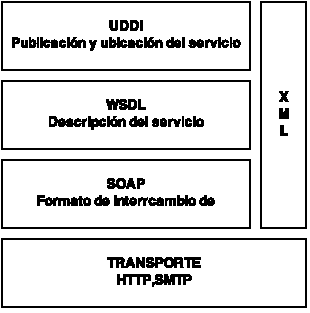
\includegraphics[scale=1]{arquitectura_ws}
    \caption{Arquitectura básica de protocolos de Web Services}
    \label{figura:arquitectura_ws}
  \end{figure}
La tecnología de Web Services está basada en tres estándares fundamentales: Simple Object
Access Protocol (SOAP) , Web Service Description Language (WSDL) y Universal
Description Discovery and Integration (UDDI) como se muestra en la figura \ref{figura:arquitectura_ws}.
\subsubsection{XML}
\label{MarcoConceptual:XML}
\emph{Extensible Markup Language (XML)} es un formato de texto simple, muy flexible derivado de SGML (ISO 8879). Originalmente diseñado para cumplir con los desafíos de la publicación electrónica a gran escala, XML también está desempeñando un papel cada vez más importante en el intercambio de una amplia variedad de datos en la Web y en otras partes. No es un lenguaje, es un metalenguaje. Permite crear lenguajes, definir etiquetas y sus atributos, definir relaciones entre las etiquetas, describir servicios \cite{XSLT:definiciones,XML:W3C}.
\subsubsection{XSLT}
\label{MarcoConceptual:XSLT}
\emph{Extensible Stylesheet Language Transformations (XSLT)} es un lenguaje de transformación de documentos \emph{XML} en otros documentos \emph{XML}.
  \begin{figure}[h]
    \centering
    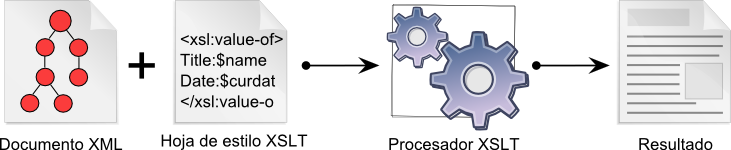
\includegraphics[scale=0.5]{xslt_resumen}
    \caption{Etapas de aplicación de un XSLT}
    \label{figura:xslt_resumen}
  \end{figure}
 Es un lenguaje de programación declarativo. El flujo de una transformación se puede notar en la figura \ref{figura:xslt_resumen}
 \begin{enumerate}
        \item Un documento XML
        \item La hoja de estilo XSLT es el documento que contiene el código fuente del programa, es decir, las reglas de transformación que se van a aplicar al documento de origen.
        \item El procesador XSLT es el programa que aplica al documento de origen, las reglas de transformación definidas en la hoja de estilo XSLT
        \item El resultado de la ejecución del programa es un nuevo documento (que puede ser un documento XML o no)
        \end{enumerate}
  \begin{figure}[h]
    \centering
    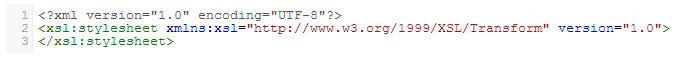
\includegraphics[scale=0.5]{xslt_ejemplo}
    \caption{Estructura básica XSLT}
    \label{figura:xslt_ejemplo}
  \end{figure}
Una hoja de estilo XSLT es un documento XML. Se utilizan etiquetas para definir estas hojas. Las etiquetas mínimas para definirla son las que se muestra en la figura \ref{figura:xslt_ejemplo}. Estas etiquetas son \cite{XSLT:definiciones}:
        \begin{enumerate}
        \item La declaración xml <?xml>, propia de cualquier documento XML
        \item La instrucción <xsl:stylesheet> es la etiqueta raíz de la hoja de estilo, sus atributos indican la versión y el espacio de nombres correspondiente
        \end{enumerate}
Dentro de la instrucción <xsl:stylesheet> se pueden encontrar los llamados elementos de alto nivel y las plantillas, como en el ejemplo siguiente \cite{XSLT:definiciones}:
  \begin{figure}[h]
    \centering
    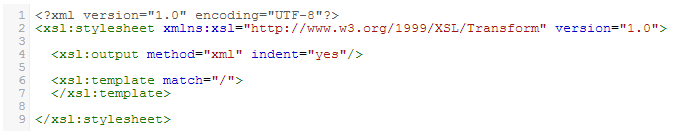
\includegraphics[scale=0.5]{xslt_ejemplo2}
    \caption{Ejemplo básico XSLT}
    \label{figura:xslt_ejemplo2}
  \end{figure}
En la figura \ref{figura:xslt_ejemplo2} se ven las etiquetas \cite{XSLT:definiciones}:
        \begin{enumerate}
        \item El elemento de alto nivel <xsl:output> indica el tipo de salida producida
        \item La instrucción <xsl:template> es una plantilla.
          \begin{enumerate}
          \item El atributo match indica los elementos afectados por la plantilla y contiene una expresión XPath
          \item El contenido de la instrucción define la transformación a aplicar (si la instrucción no contiene nada, como en el ejemplo anterior, sustituirá el nodo por nada)
          \end{enumerate}
        \end{enumerate}
A través de un \emph{XML Schema} se establece la estructura detallada de los mensajes definiendo qué elementos y atributos se permiten, en qué orden deben aparecer y qué tipo de datos pueden contener \citep{Tesis:LauraGonzalez:PlataformaESB,XML:W3C}.
\subsubsection{SOAP}
\label{MarcoConceptual:SOAP}
\emph{Simple Object Access Protocol (SOAP)} es un formato de mensaje XML utilizado en interacciones de servicios web. Los mensajes SOAP habitualmente se envían sobre HTTP o JMS, pero se pueden utilizar otros protocolos. El uso de SOAP en un servicio web específico se describe mediante la definición WSDL. SOAP no pone restricciones sobre la semántica de los mensajes de intercambio, no se encarga de cuestiones de fiabilidad,integridad de los mensajes, transacciones, seguridad, etc \cite{WebServices:CCIA}.
  \begin{figure}[h]
    \centering
    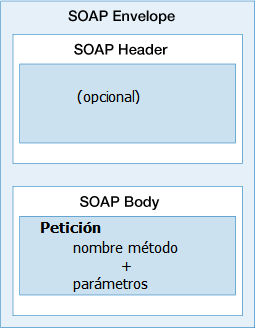
\includegraphics[scale=0.5]{mensaje_soap}
    \caption{estructura de un mensaje SOAP}
    \label{figura:mensaje_soap}
  \end{figure}
En la figura \ref{figura:mensaje_soap} se puede observar la estructura de los mensajes SOAP. Consiste en un \emph{envelope} que contiene una cabecera \emph{(etiqueta <Header>)} que es un componente opcional que brinda la información sobre el mensaje a usar por la infraestructura del Web Services; y el otro componente es el cuerpo \emph{(etiqueta <Body>)} que es obligatorio donde contiene información específica a usar por las aplicaciones que usan o implementan el Web Services. Los extremos son responsables de acordar el formato de la información intercambiada y de generar y/o procesar su contenido \cite{WebServices:CCIA}.
  \begin{figure}[h]
    \centering
    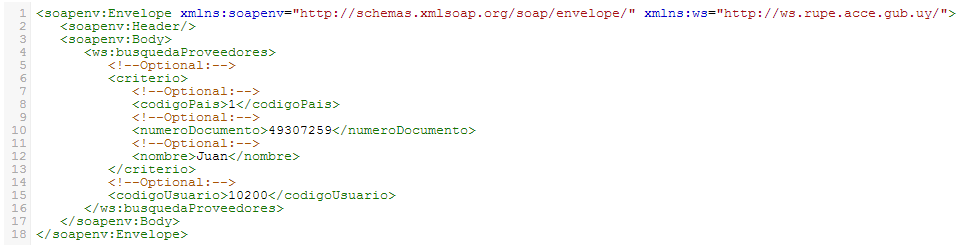
\includegraphics[scale=0.5]{ej_mensaje_soap}
    \caption{Ejemplo de mensaje SOAP}
    \label{figura:ej_mensaje_soap}
  \end{figure}
La figura \ref{figura:ej_mensaje_soap} es un ejemplo de un mensaje SOAP invocando a la operación \emph{busquedaProveedores} con los parámetros \emph{codigoPais, numeroDocumento, nombre y CodigoUsuario}.
  \begin{figure}[h]
    \centering
    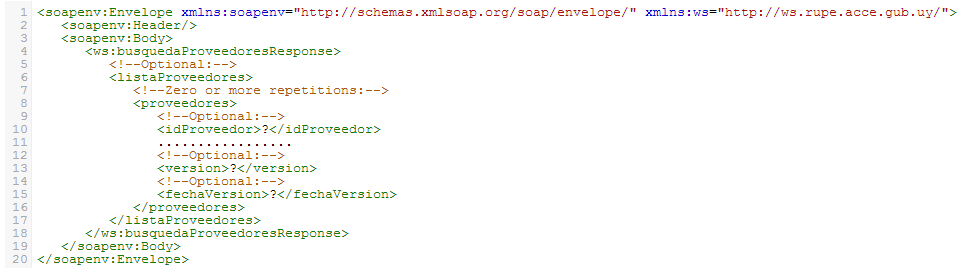
\includegraphics[scale=0.5]{ej_resp_mensaje_soap}
    \caption{Ejemplo de respuesta mensaje SOAP}
    \label{figura:ej_resp_mensaje_soap}
  \end{figure}
Como resultado de la invocación, se recibe un mensaje como representa la figura \ref{figura:ej_resp_mensaje_soap}.
\subsubsection{WSDL}
\label{MarcoConceptual:WSDL}
\emph{Web Services Description Language (WSDL)} permite describir los distintos métodos o funciones que están disponibles en un Web Services, con sus parámetros o argumentos que se les debe pasar y el tipo de dato que retornará la función como resultado, y las ubicaciones en donde puede accederse. Especifica la sintaxis y los mecanismos de intercambio de mensajes \cite{WSDL:W3C}. \emph{WSDL} es es un lenguaje de definición de interfaces basado en XML que permite describir de forma estándar a los Web Services \cite{Tesis:LauraGonzalez:PlataformaESB} y representa una especie de contrato entre el proveedor y el que solicita.
Dentro de la definición del \emph{WSDL} se encuentra el \emph{endpoint} el cual nos indica una localización específica para acceder a un Web Services usando un protocolo y formato de datos específico.

  \begin{figure}[h]
    \centering
    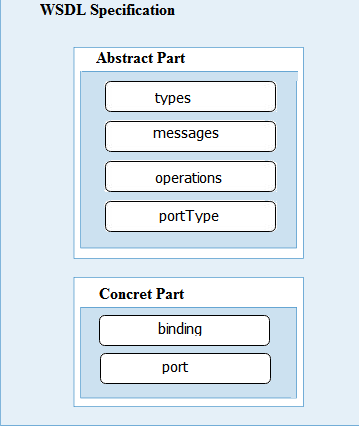
\includegraphics[scale=0.5]{estructura_wsdl}
    \caption{Estructura WSDL}
    \label{figura:estructura_wsdl}
  \end{figure}
En la figura \ref{figura:estructura_wsdl} se puede observar la estructura definida por un \emph{WSDL}.
La \emph{descripción abstracta} contiene \cite{WSDL:W3C}
				\begin{enumerate}
				\item \emph{Types} para indicar los tipos de datos que utiliza el Web Service
				\item \emph{Message} representa una definición abstracta de los datos transmitidos
				\item \emph{PortType} es un conjunto de operaciones abstractas. Cada operación refiere a mensajes de salida y entrada
				\end{enumerate}
En la \emph{descripción concreta} se encuentran los elementos \cite{WSDL:W3C} 
				\begin{enumerate}
				\item \emph{Binding} especifica un protocolo concreto así como el formato de datos para las operaciones, y los mensajes definidos en un portType particular. Puede existir
cualquier número de bindings para un portType
				\item \emph{Port} especifica una dirección para un \emph{binding}. Define un \emph{endpoint} particular especificando una dirección única para un binding. refiere a mensajes de salida y entrada
				\end{enumerate}
\subsubsection{UDDI}
\label{MarcoConceptual:UDDI}
\emph{Universal description, discovery, and integration (UDDI)} es la especificación de una
plataforma estándar interoperable que permite publicar, encontrar y utilizar Web Services
de forma rápida, sencilla y dinámica a través de Internet \cite{UDDI:def}.

\section{Gobernanza en SOA}
  \label{MarcoConceptual:GobernanzaSOA}

  La \emph{gobernanza en arquitecturas orientadas a servicios (SOA)}, es la tarea de administración de una SOA: brinda las reglas para la toma de decisiones, establece los procesos necesarios, define los roles que forman parte del sistema administrativo y establece las métricas que determinan el ajuste de la toma de decisiones a las reglas establecidas. La gobernanza no dice cuándo ni cómo tomar una decisión; determina quién debería hacerlo y establece los límites para esa persona o grupo. \cite{Erl:2011:SGG:1983453}

  \begin{figure}[h]
    \centering
    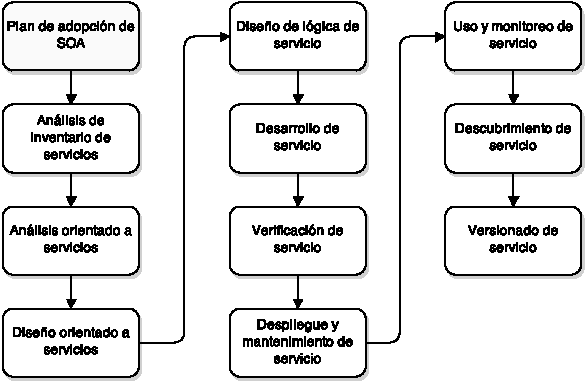
\includegraphics[scale=0.5]{ciclo_de_vida_del_proyecto}
    \caption{Etapas comunes de un proyecto SOA}
    \label{figura:ciclo_de_vida_del_proyecto}
  \end{figure}

  La figura \ref{figura:ciclo_de_vida_del_proyecto} muestra las etapas comunes de un proyecto SOA las cuales son también etapas del \emph{ciclo de vida} de los servicios.

  Todo proyecto SOA comienza con un plan de adopción. En este se aborda el alcance del proyecto (visión general de qué servicios serán incluidos), metas, tiempos de ejecución, sistema de gobernanza, forma de financiación, entre otros.

  Una vez establecidos los parámetros para la adopción de una SOA, comienza el análisis para la identificación de los servicios que compondrán la arquitectura. Una característica fundamental de los proyectos SOA es el \emph{análisis por adelantado} en la identificación de los servicios. Un servicio pobremente analizado en etapas tempranas, concluirá en una implementación poco efectiva, mientras que un análisis en profundidad brindará mayor información para un diseño adecuado que generará beneficios para la organización en términos de la SOA.

  La primer etapa de análisis corresponde al \emph{análisis de inventarios de servicios}. El objetivo en esta etapa es definir «blueprints» o planos (cianotipos) que describen las características de un conjunto de servicios que serán incluidos finalmente en dicho inventario. Se trata de una etapa de análisis que abarca un ciclo de definiciones acotadas a cada servicio, y que en cada iteración refinan el blueprint del inventario. Un blueprint permite normalizar los servicios incluidos dentro de un inventario de manera que estos no se superpongan, maximizando la reutilización y la separación de responsabilidades entre servicios del mismo inventario. \cite{Erl:2011:SGG:1983453}

  \begin{quote}
    ``Un inventario representa una colección de servicios independientemente estandarizados y gobernados''. \cite{Erl:2011:SGG:1983453}
  \end{quote}

  No solo la calidad de los servicios en forma individual depende de la profundiad del análisis por adelantado, sino también la de los blueprints, y como consecuencia, la de los inventarios y sus servicios en último lugar.

  Las etapas siguientes al análisis involucran el diseño, implementación y puesta en producción de cada servicio por separado. En la sección \ref{Apendices:ApendiceA} se incluye una descripción extendida acerca de las etapas comunes de un proyecto SOA siguiendo los lineamientos del texto de base.

  En un caso ideal, los inventarios están relacionados directamente con algún \emph{dominio} o línea de negocios de la organización. Es esperable que estos dominios —cuando son más de uno— estén a cargo de un propietario dentro de la organización, quien los gobierna u administra. En grandes proyectos, la cantidad de dominios y propietarios —y la relación existente entre ellos— puede resultar propicia para establecer una jerarquía de gobernanza de los mismos que permita establecer criterios adecuados para cada conjunto, y a la vez, que estos estén alineados con los objetivos generales de gobernanza del proyecto SOA.

  La entidad reguladora de estos dominios dentro de la organización es la \emph{oficina del programa de gobernanza en SOA} (SGPO, por sus siglas en Inglés). Una SGPO es un área encargada de uno o más dominios de servicios dentro de la organización, según el modelo de jurisdicción adoptado por el sistema de gobernanza. En una organización dada, múltiples SGPO pueden coexistir en base a los dominios identificados y sus propietarios.

  \begin{table}[h]
    \begin{tabular}{p{0.25\linewidth} | p{0.75\linewidth}}
      \textbf{Tipo} & \textbf{Descripción} \\
      \hline
      SGPO empresarial centralizada & Única SGPO encargada de un único dominio de servicios de la organización\\
      \hline
      SGPO con dominios centralizados & Distintos dominios estandarizados son abarcados por un único sistema de gobernanza dirigido por una SGPO central.\\
      \hline
      SGPO con dominios federados & Varias SGPO responsables de un dominio cada una donde llevan a cabo su propio sistema de gobernanza, el cual debe cumplir con lineamientos introducidos por una SGPO central\\
      \hline
      SGPO con dominios independientes & SGPO individuales responsables de un dominio cada una donde aplican el sistema de gobernanza en forma independiente.\\
      \hline
    \end{tabular}
    \caption{Modelos de jurisdicción de SGPO}
    \label{tabla:modelos_sgpo}
  \end{table}

  \begin{figure}[h]
    \centering
    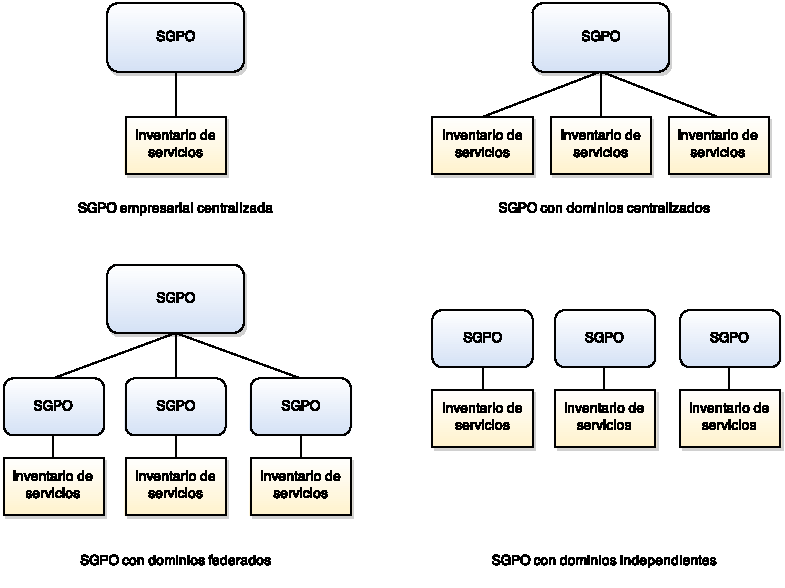
\includegraphics[scale=0.5]{modelos_sgpo}
    \caption{Representación gráfica de modelos de jurisdicción de SGPO \cite{Erl:2011:SGG:1983453}}
    \label{imagen:modelos_sgpo}
  \end{figure}

  En el cuadro \ref{tabla:modelos_sgpo} y figura \ref{imagen:modelos_sgpo} se describen los distintos modelos de jurisdicción de SGPO básicos aplicables a una organización.

\section{Versionado}
\label{MarcoConceptual:versionado}

\section{Calidad en Servicios}
\label{MarcoConceptual:calidad}
La \emph{calidad de los servicios (QoS)} es un elemento importante que permite determinar el rendimiento, utilidad y facilidad de uso de los mismos, entre otros factores.
Se utiliza normalmente para describir las características no funcionales de los web services y como criterio para la evaluación de los diferentes web services.
Cada servicio debe cumplir con un contrato escrito entre el proveedor del mismo y el cliente, donde se define un \emph{acuerdo de nivel de servicio (SLA)} en el cual el proveedor debe respetar todos los criterios de calidad que se compromete a cumplir. \cite{Bool:QoSWS}

\subsection{Metamodelo de calidad}
\label{MarcoConceptual:metamodelo_calidad}
Un metamodelo de calidad permite definir distintos niveles para evaluar la calidad de un servicio. El metamodelo básico es \emph{"Quality Abstract"} que contiene la siguiente estructura.  \cite{InCo:Seminario}
  \begin{figure}[h]
    \centering
    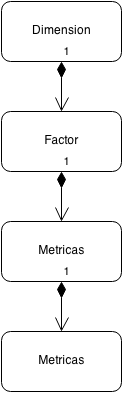
\includegraphics[scale=0.8]{metamodelo_de_calidad}
    \caption{Metamodelo Abstracto de Calidad}
    \label{figura:metamodelo_de_calidad}
  \end{figure}

La figura \ref{figura:metamodelo_de_calidad} nos indican los siguientes niveles.

			\begin{enumerate}
				\item Dimensión: Es el aspecto de la calidad correspondiente a la perspectiva que brinda el mayor nivel de abstracción de la misma \cite{InCo:Seminario}.
				\item Factor: Se ubica en el nivel inmediato inferior a la dimension por lo que corresponde a un aspecto particular de la dimension de la calidad. Un factor pude ser mas adecuado que otro para algún tipo de problema o aplicación que se este analizando.
				\item Métrica: La métrica corresponde a un instrumento que define una forma de medir un factor de calidad.\cite{InCo:Seminario}Puede haber diferentes métricas para el mismo factor, las cuales miden el factor desde diferentes puntos de vista. Consta de tres elementos que tienen que estar bien definidos
				\begin{enumerate}
				\item Semántica (define como se mide la métrica, le da significado)
				\item Unidad de medida (es la cantidad en términos de magnitud o porcentaje)
				\item Granularidad de la medida (especificidad a la que se define un nivel de detalle)
				\end{enumerate}
				\item Método: El método corresponde al proceso por el cual se implementa la métrica. Puede haber más de un método que implemente la misma métrica. La implementación del método depende del dominio de la aplicación en concreto y de aspectos de bajo nivel como pueden ser la estructura de datos que es objeto de estudio.
			\end{enumerate}


\subsection{Modelos de Calidad}
\label{MarcoConceptual:modelos_calidad}
Un \emph{modelo de calidad} es el resultado de definir que elementos del metamodelo se quiere analizar. Esos elementos son los factores de calidad que son de interés monitorear su comportamiento para cada servicio. Existen varios enfoques interesantes de modelos, particularmente se analizarán el Modelo de Calidad para Web Services de OASIS, el Modelo de calidad en base al proyecto S-Cube y los principales factores de calidad que son requeridos para apoyar la QoS por IBM.
\subsubsection{Modelo OASIS}
\label{MarcoConceptual:modelo_OASIS}
\emph{OASIS (Organization for the Advancement of Structured Information Standards)} es una organización sin fines de lucro que conduce el desarrollo, unificación y adopción de estándares para la sociedad de información global. Ha producido muchos de los estándares hoy usados para web services \cite{OASIS:def}.Presenta un modelo conceptual que define la interacción entre las partes involucradas \emph{Actores de calidad (Quality Associates)}, \emph{Actividades de calidad (Quality Activities)} y \emph{Factores de calidad (Quality Factors)} para habilitar la calidad de servicio.
  \begin{figure}[h]
    \centering
    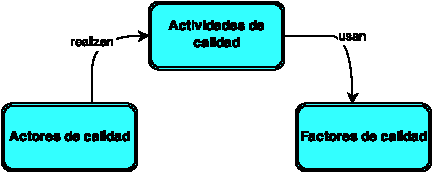
\includegraphics[scale=1]{oasis_modelo}
    \caption{Modelo Conceptual de Calidad para Web Services OASIS}
    \label{figura:oasis_modelo}
  \end{figure}
En la figura \ref{figura:oasis_modelo} se muestra el modelo conceptual de OASIS. Por ejemplo, un consumidor y un proveedor de Web Services \emph{(actores de calidad)} pueden establecer un Acuerdo de Nivel de Servicio \emph{(actividad de calidad)}, que involucre el tiempo de respuesta y la disponibilidad de los servicios \emph{(factores de calidad)} \cite{Tesis:LauraGonzalez:PlataformaESB}.
Al realizar un mapeo con el metamodelo abstracto de calidad visto en la sección \ref{MarcoConceptual:modelo_OASIS}, vemos en la figura \ref{figura:metamodelo_de_calidad} la agrupación del modelo propuesto por OASIS en la estructura Dimensión - Factor - Métrica \cite{Articulo:LauraGonzalez:CalidadWS}.
  \begin{figure}[h]
    \centering
    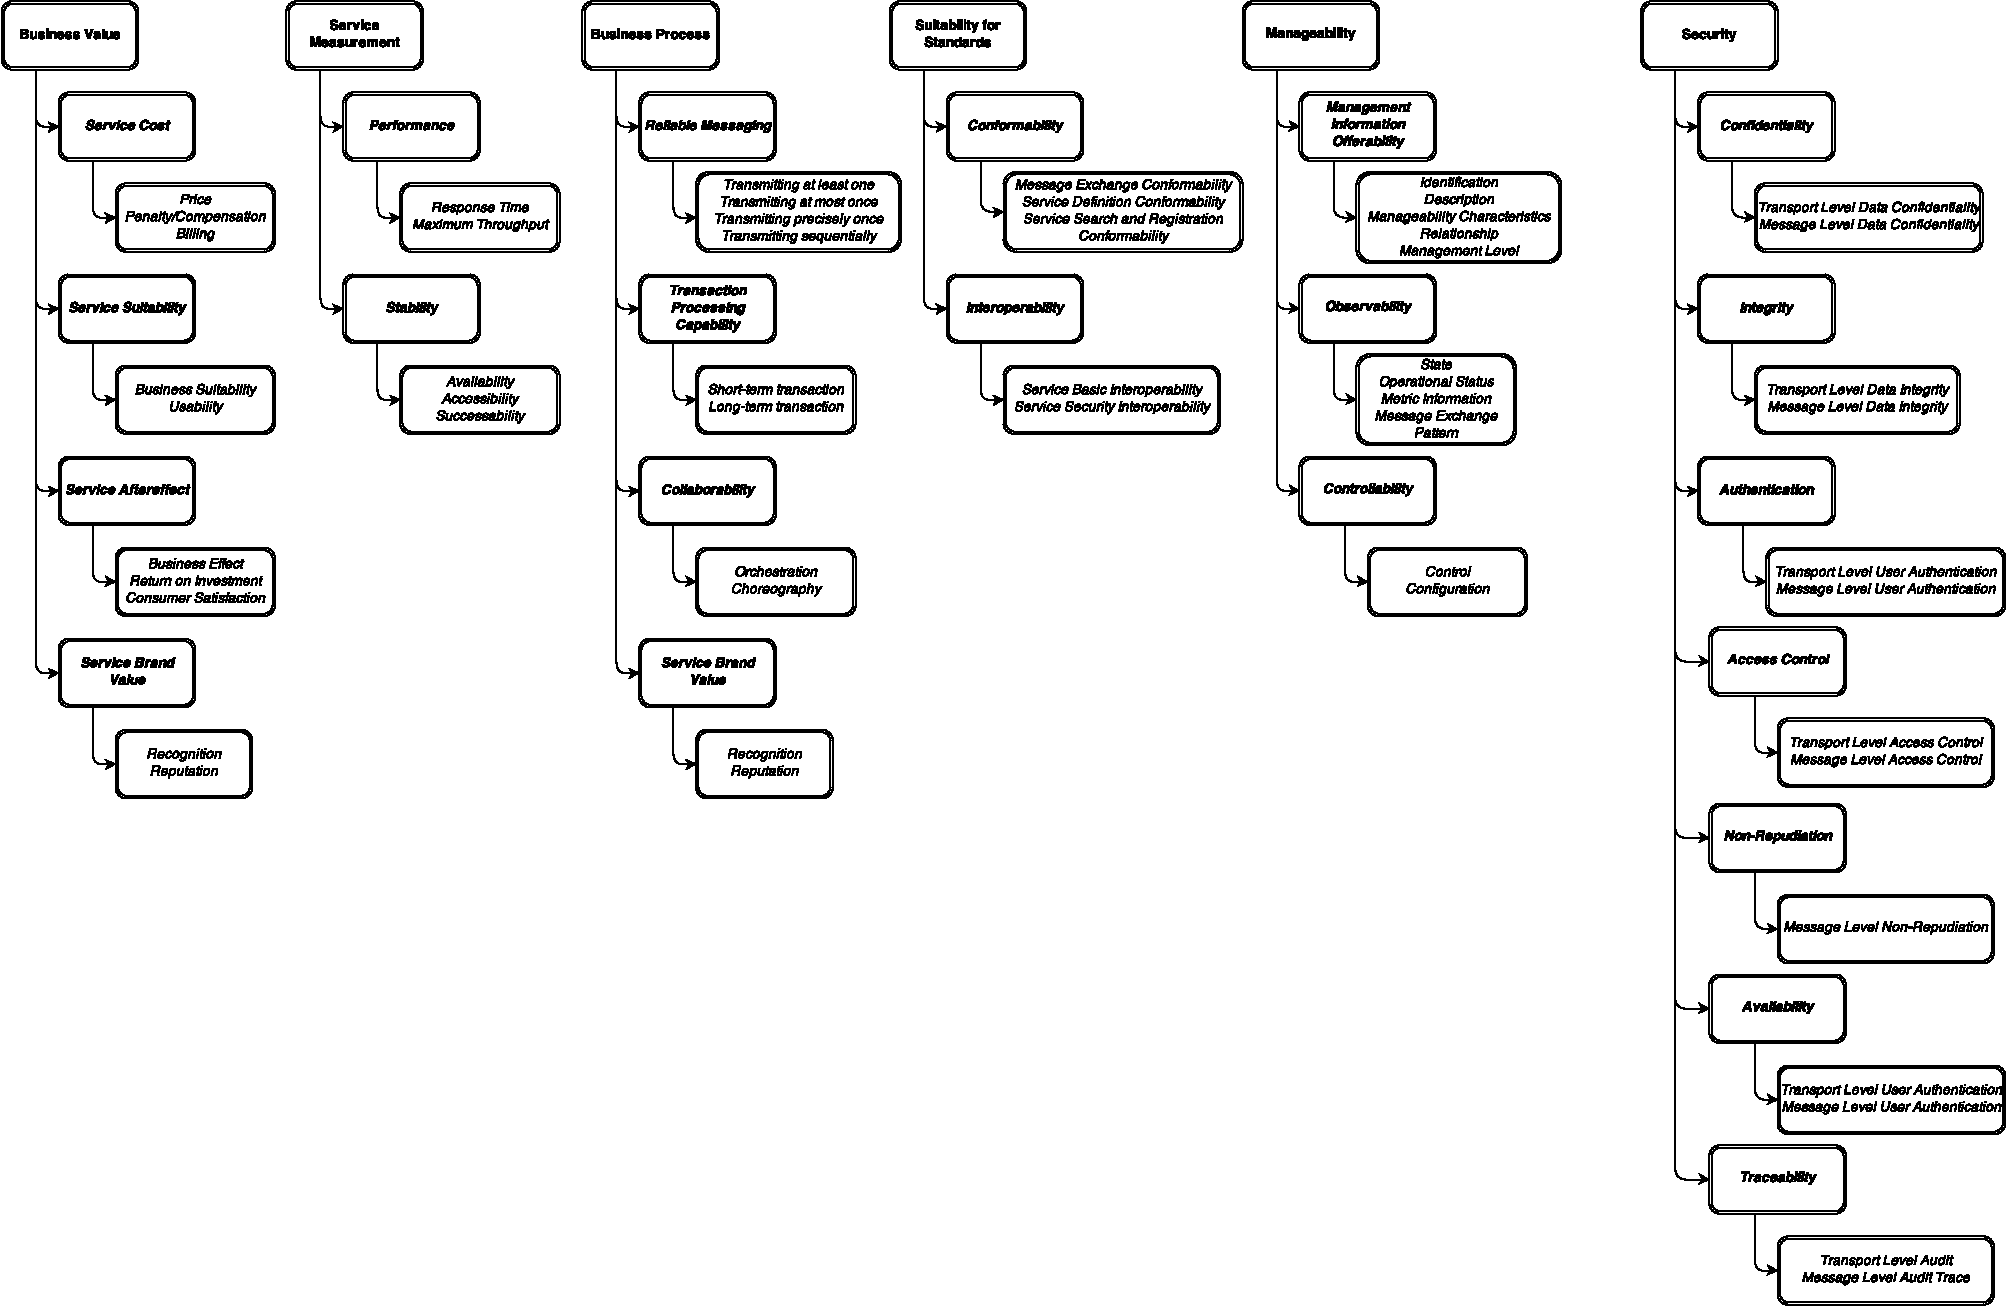
\includegraphics[scale=0.5]{metamodelo_OASIS}
    \caption{Metamodelo de Calidad propuesto por OASIS}
    \label{figura:metamodelo_OASIS}
  \end{figure}
En el Anexo se describen cada una de las métricas del modelo.

\subsubsection{Modelo S-Cube}
\label{MarcoConceptual:modelo_SCube}
S-Cube es un proyecto Europeo que define  principios, técnicas y métodos  para asegurar la calidad de los servicios. Diseñó un modelo de calidad para sistemas basados en servicios seleccionado distintos modelos de diferentes disciplinas, seleccionando los atributos de calidad relevante para los asegurar la calidad en los servicios \cite{Scube}.
  \begin{figure}[h]
    \centering
    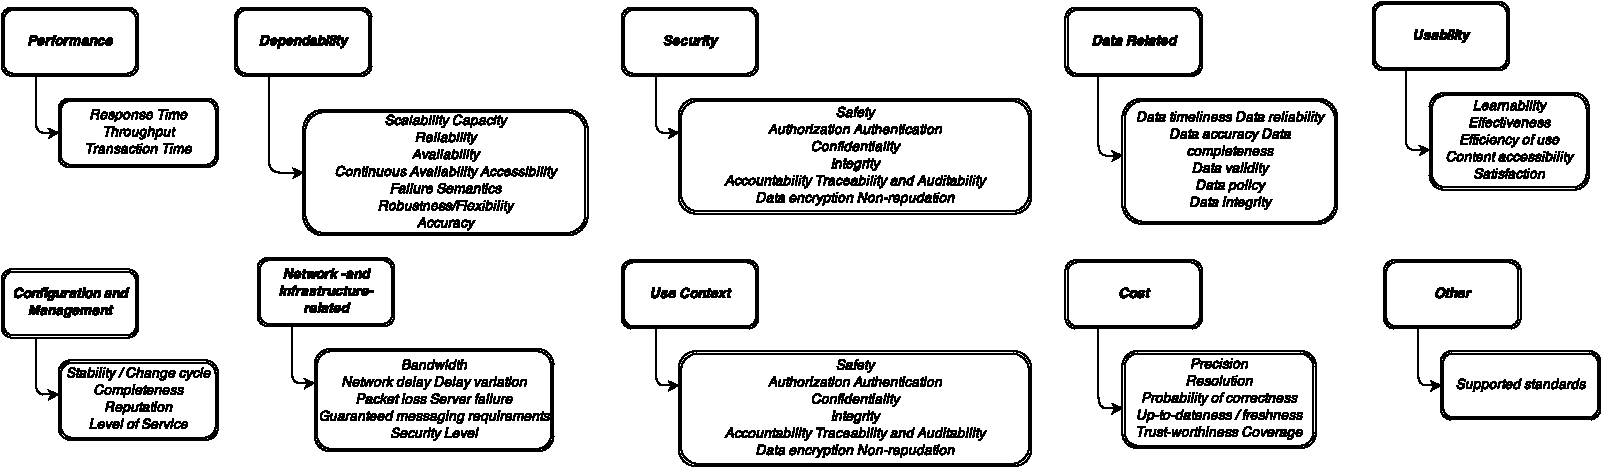
\includegraphics[scale=0.60]{modelo_Scube}
    \caption{Modelo de Calidad S-Cube}
    \label{figura:modelo_Scube}
  \end{figure}
Una vez concluida la elección de atributos, se agrupan en categorías y forman el modelo presentado en la figura \ref{figura:modelo_Scube}. 
\cite{Articulo:LauraGonzalez:CalidadWS}.
En el Anexo se describen cada una de las métricas del modelo.
\subsubsection{Modelo IBM}
\label{MarcoConceptual:modelo_IBM}
\emph{International Business Machines (IBM)} es una empresa multinacional estadounidense de tecnología y consultoria. IBM fabrica y comercializa hardware y software para computadoras, y ofrece servicios de infraestructura, alojamiento de Internet, y consultoría en una amplia gama de áreas relacionadas con la informática. Con la evolución de los Web Services, IBM analiza los principales requisitos de calidad que se deben monitorear en los servicios \cite{IBM:QoS}.
  \begin{figure}[h]
    \centering
    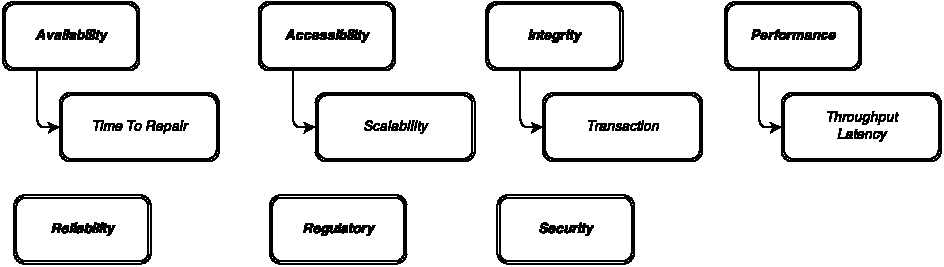
\includegraphics[scale=0.9]{modeloIBM}
    \caption{Modelo de calidad IBM}
    \label{figura:modelo_IBM}
  \end{figure}
En la figura \ref{figura:modelo_IBM} se muestran los factores de calidad que propone IBM para un modelo de calidad. En el Anexo se describen cada una de las métricas del modelo.
